\documentclass[12pt,english,dvipsnames]{beamer}
\usetheme{CambridgeUS}
\usecolortheme{beaver}
\setbeamersize{text margin left=.5cm,text margin right=.5cm}
\setbeamertemplate{navigation symbols}{}

\setlength{\paperheight}{21.0cm}
\setlength{\paperwidth}{29.7cm}
\setlength{\textheight}{20.0cm}
\setlength{\textwidth}{28.7cm}  

\usepackage[utf8]{inputenc}
% \usepackage{default}
\usepackage{colortbl}
\usepackage{graphicx}
\usepackage{tikz}
\usepackage{color}
\usepackage[english]{babel}
\usepackage{hyperref}
\usepackage{listings}
\usepackage{fancyvrb}
\usepackage{pgffor}
\usepackage{intcalc}
\usepackage{python}

%====================================================================================================
\definecolor{lightGreenYellow}{rgb}{0.92,0.96,0.69}
\definecolor{lighterUAbrown}{rgb}{0.867,0.824,0.737}
\definecolor{lightUAbrown}{rgb}{0.87,0.75,0.52}
\definecolor{UAbrown}{rgb}{0.87,0.57,0.0}
\definecolor{darkUAbrown}{rgb}{0.70,0.40,0.0}
\definecolor{darkerUAbrown}{rgb}{0.50,0.28,0.0}
\definecolor{lightUAblue}{rgb}{0.32,0.37,0.40}
\definecolor{UAblue}{rgb}{0.0,0.45,0.65}
\definecolor{darkUAblue}{rgb}{0.0,0.20,0.35}
\definecolor{lightUAred}{rgb}{0.58,0.40,0.46}
\definecolor{UAred}{rgb}{0.58,0.03,0.19}
\definecolor{lightUAcyan}{rgb}{0.47,0.71,0.78}
\definecolor{UAcyan}{rgb}{0.0,0.60,0.78}
\definecolor{lightGray}{rgb}{0.98,0.94,0.98}
\definecolor{shade1}{rgb}{0.90,0.95,0.98}
\definecolor{shade2}{rgb}{0.90,0.98,0.90}
\definecolor{light1}{cmyk}{0.0,0.0,0.02,0.1}
\definecolor{light2}{cmyk}{0.05,0.0,0.1,0.0}
\definecolor{cyan}{cmyk}{1,0.0,0.0,0.0}

\definecolor{color1}{cmyk}{1.0,0.275,0.0,0.573}
\definecolor{color2}{cmyk}{0.0,0.850,0.649,0.424}
\definecolor{color3}{cmyk}{1.0,0.155,0.0,0.290}
\definecolor{color4}{cmyk}{0.0,0.258,0.949,0.224}
\setbeamercolor{palette tertiary}{fg=white,bg=color1!80}
\setbeamercolor{palette secondary}{fg=color1}
\setbeamercolor{palette primary}{fg=color1}
\setbeamercolor{block body}{fg=color1}
\setbeamercolor{title}{fg=color2}
\setbeamercolor{titlelike}{fg=color2}
% \setbeamercolor{palette secondary}{fg=color1}
% \setbeamercolor{palette secondary}{use=structure,fg=structure.fg!100!color2}
% \setbeamercolor{palette tertiary}{use=structure,fg=structure.fg!100!color3}

%====================================================================================================
\newcommand{\twotoponebottom}[6]{\begin{minipage}{#1\textwidth}#4\end{minipage}\hfill\begin{minipage}{#2\textwidth}#5\end{minipage}\vskip 1em\begin{minipage}{#3\textwidth}#6\end{minipage}}
\newcommand{\hortwo}[4]{\begin{minipage}{#1\textwidth}#3\end{minipage}\hfill\begin{minipage}{#2\textwidth}#4\end{minipage}}
\newcommand{\horthree}[6]{\begin{minipage}{#1\textwidth}#4\end{minipage}\hfill\begin{minipage}{#2\textwidth}#5\end{minipage}\hfill\begin{minipage}{#3\textwidth}#6\end{minipage}}
\newcommand{\horfour}[8]{\begin{minipage}{#1\textwidth}#5\end{minipage}\hfill\begin{minipage}{#2\textwidth}#6\end{minipage}\hfill\begin{minipage}{#3\textwidth}#7\end{minipage}\hfill\begin{minipage}{#4\textwidth}#8s\end{minipage}}
\newcommand{\vertwo}[4]{\begin{minipage}{#1\textwidth}#3\end{minipage}\vskip 0em\begin{minipage}{#2\textwidth}#4\end{minipage}}
\newcommand{\verthree}[6]{\begin{minipage}{#1\textwidth}#4\end{minipage}\vskip 0em\begin{minipage}{#2\textwidth}#5\end{minipage}\vskip 0em\begin{minipage}{#3\textwidth}#6\end{minipage}}

\newcommand{\bi}{\begin{itemize}}
\newcommand{\ei}{\end{itemize}}   
\newcommand{\bbl}[1]{\begin{block}{#1}}
\newcommand{\ebl}{\end{block}}   
\newcommand{\forcespace}{\mbox{\ }}

\newcommand{\ra}[0]{\ensuremath{\rightarrow} }
\newcommand{\as}[0]{\ensuremath{\alpha\_S} }

\newcommand{\mind}[1]{\LARGE\textbf{\textsc{\color{red}{#1}}}\normalsize}

%====================================================================================================
\tikzset{overlayblock/.style={draw=UAred, text=UAred, rounded corners=1mm, align=justify, fill=gray!30, text opacity=0.8, fill opacity=0.6}}
\tikzset{overlayblockbare/.style={text=Black, rounded corners=0mm, align=justify, text opacity=1.0}}
\tikzset{overlayblockframe/.style={draw=Red, text=Red, rounded corners=1mm, align=justify, text opacity=1.0}}
\tikzset{overlayblockred/.style={draw=Red, text=Red, rounded corners=1mm, align=justify, fill=gray!30, text opacity=0.8, fill opacity=0.6}}
\tikzset{overlayblocksimple/.style={draw=Black, text=Black, rounded corners=0mm, align=justify, text opacity=1.0}}
\newcommand{\overlay}[3]{\begin{tikzpicture}[overlay, remember picture]\pgftransformshift{\pgfpointanchor{current page}{center}}\node<#1$>$[overlayblock] at #2 {#3};\end{tikzpicture}}
\newcommand{\overlaybare}[3]{\begin{tikzpicture}[overlay, remember picture]\pgftransformshift{\pgfpointanchor{current page}{center}}\node<#1$>$[overlayblockbare] at #2 {#3};\end{tikzpicture}}
\newcommand{\overlayframe}[3]{\begin{tikzpicture}[overlay, remember picture]\pgftransformshift{\pgfpointanchor{current page}{center}}\node<#1$>$[overlayblockframe] at #2 {#3};\end{tikzpicture}}
\newcommand{\overlayred}[3]{\begin{tikzpicture}[overlay, remember picture]\pgftransformshift{\pgfpointanchor{current page}{center}}\node<#1$>$[overlayblockred] at #2 {#3};\end{tikzpicture}}
\newcommand{\overlaysimple}[3]{\begin{tikzpicture}[overlay, remember picture]\pgftransformshift{\pgfpointanchor{current page}{center}}\node<#1$>$[overlayblocksimple] at #2 {#3};\end{tikzpicture}}

\newcommand{\addpic}[2]{\includegraphics[width=#1\textwidth]{{#2}}}
\newcommand{\addpich}[2]{\includegraphics[height=#1\textwidth]{{#2}}}
\newcommand{\addpicc}[3]{\begin{figure}\includegraphics[width=#1\textwidth]{{#2}}\caption{#3}\end{figure}}


%====================================================================================================
\newcommand{\backupbegin}{
   \newcounter{framenumberappendix}
   \setcounter{framenumberappendix}{\value{framenumber}}
}
\newcommand{\backupend}{
   \addtocounter{framenumberappendix}{-\value{framenumber}}
   \addtocounter{framenumber}{\value{framenumberappendix}} 
}
%====================================================================================================
\let\OldItem\item
\let\OldSubItem\subitem
\newcommand{\itemTwo}{%
    \setbeamertemplate{itemize item}[triangle]
    \setbeamercolor{itemize item}{fg=darkUAblue}
    \color{darkUAblue}
    \OldItem%
    \def\nextitem{\itemOne}%
}%
\newcommand{\itemOne}{%
    \setbeamertemplate{itemize item}[triangle]
    \setbeamercolor{itemize item}{fg=UAblue}
    \color{UAblue}
    \OldItem%
    \def\nextitem{\itemTwo}%
}%
\newcommand{\subItemTwo}{%
    \setbeamertemplate{itemize subitem}[triangle]
    \setbeamercolor{itemize subitem}{fg=darkerUAbrown}
    \color{darkerUAbrown}
    \OldItem%
    \def\nextsubitem{\subItemOne}%
}%
\newcommand{\subItemOne}{%
    \setbeamertemplate{itemize subitem}[triangle]
    \setbeamercolor{itemize subitem}{fg=darkUAbrown}
    \color{darkUAbrown}
    \OldItem%
    \def\nextsubitem{\subItemTwo}%
}%
\newcommand{\nextitem}{\itemOne}%
\newcommand{\nextsubitem}{\subItemOne}
\newcommand*{\AlternateColors}{%
    \def\item{\nextitem}%
    \def\subitem{\nextsubitem}
}%
%====================================================================================================
\newcommand{\UAoverlay}[0]{%
\begin{tikzpicture}[remember picture,overlay,shift={(current page.north east)}]
\node (zero) at (-1.8cm,-0.93cm) {\includegraphics[width=1cm]{../logos/CMS.pdf}\hspace{0.15cm}\includegraphics[width=1cm]{../logos/CERN.pdf}\hspace{0.15cm}\includegraphics[width=1cm]{../logos/UA.pdf}}; 
\end{tikzpicture}
}

%====================================================================================================
\author[S. Alderweireldt]{Sara Alderweireldt}
\date{\today}
\institute[UA]{\small Universiteit Antwerpen}
\title{VBFHbb}

\begin{document}
\lstset{language=bash,frame=single,numbers=left,numbersep=5pt,stepnumber=2,numberstyle=\tiny\color{blue},breaklines=true,numberfirstline=true}
%====================================================================================================
% \begin{frame}%\UAoverlay
% \maketitle
% \end{frame}
\section{\footnotesize Selection and distribution in signal}
\begin{frame}[t,fragile]%\UAoverlay
\footnotesize
full selection + trigger: 
\begin{itemize}
 \item mqq[2] $>$ XXX \&\& mjjTrig $>$ XXX
 \item dEtaqq[2] $>$ 3.5 \&\& dEtaTrig $>$ 3.5
 \item ptAve $>$ 80
 \item jetPt[3] $>$ 30\vskip 1em
 \item triggerResult[9] == 1\vskip 2em
\end{itemize}

\includegraphics[width=0.48\textwidth]{/home/salderwe/UA/svncontrolled/2013/vbfHbb/vbfHbb_git/trigger/signal_distribution-mqq2_dEtaqq2.pdf}\hfill
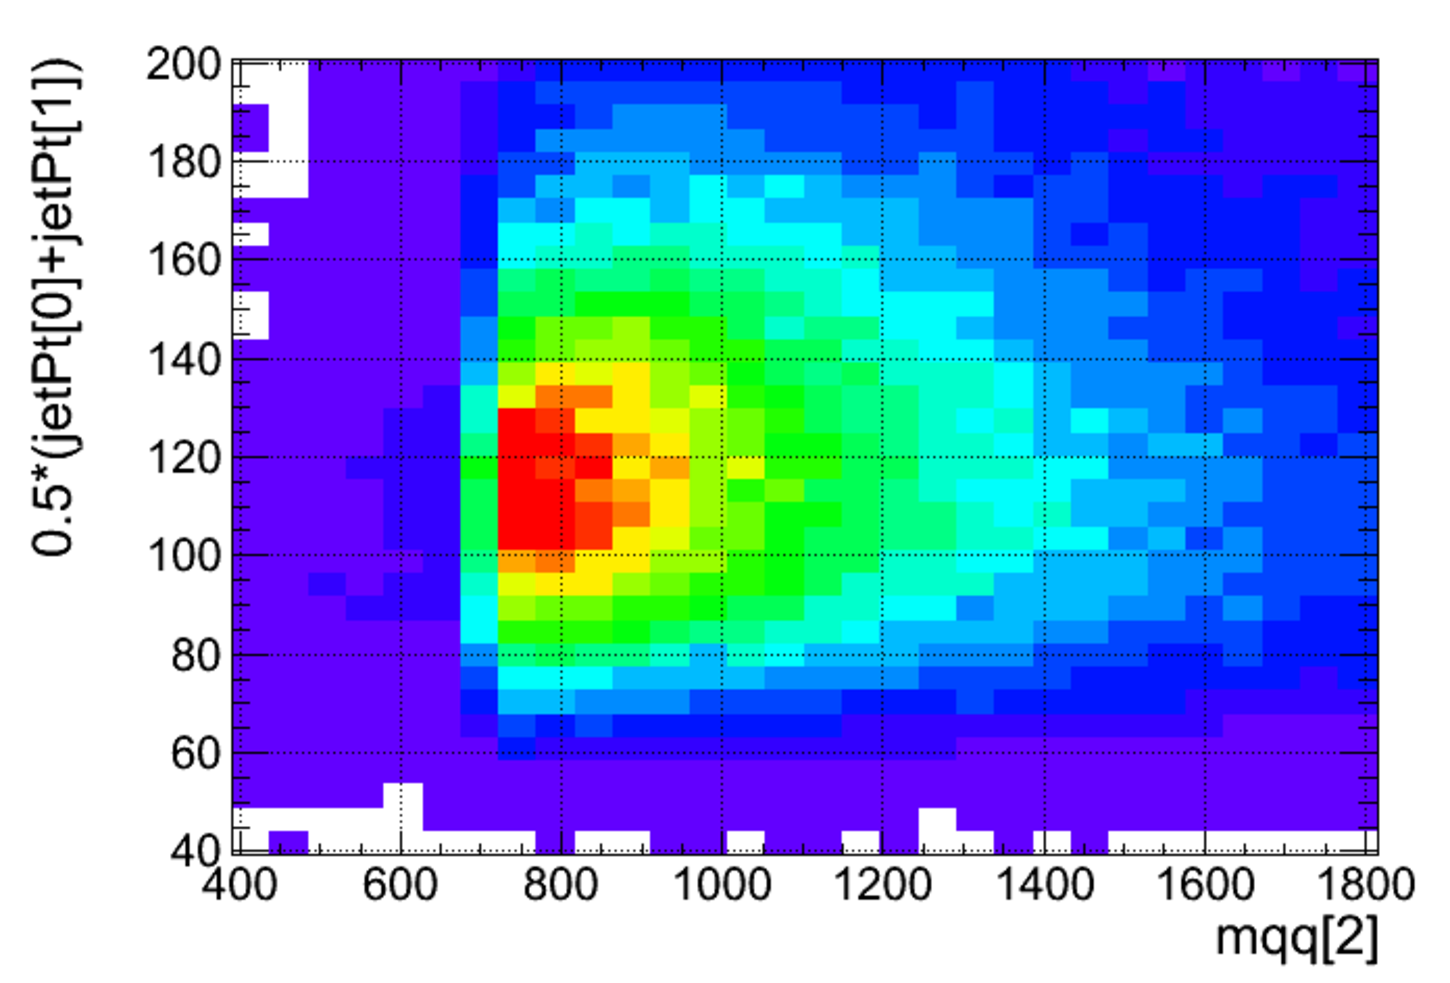
\includegraphics[width=0.48\textwidth]{./Kostas/2DSig.pdf}

\end{frame}
%====================================================================================================
\section{\tiny UNCORRECTED (mqq[2]$>$700)\&\&(dEtaqq[2]$>$3.5)\&\&(mjjTrig$>$700) \&\&(dEtaTrig$>$3.5)\&\&(0.5*(jetPt[0]+jetPt[1])$>$80)\&\&(jetPt[3]$>$30.)}
% \setbeamercolor{background canvas}{bg=Cyan!25}
\begin{frame}[t,fragile]%\UAoverlay
\begin{python}
import glob
directory = "/home/salderwe/UA/svncontrolled/2013/vbfHbb/vbfHbb_git/trigger/plots/trigger_Nmin1_20140128/LUMI-PU.3-XSEC/turnonCurves/global_global/sdEtaTrig_gt3p5-dEtaqq2_gt3p5-jetPt3_gt30-jetPtAve_gt80-mjjTrig_gt700-mqq2_gt700-run194270_tVBF"
plots = glob.glob("%s/*.png"%directory) 
for ii,i in enumerate(sorted(plots)):
  print r"\includegraphics[width=0.28\textwidth]{%s}"%i
  if ii%3==2: print r"\newline"
  else: print r"\hfill"
for jj in range(ii,9):
  print r"
\includegraphics[width=0.28\textwidth]{./blank.pdf}"
  if jj%3==2: print r"\newline"
  else: print r"\hfill"
\end{python}

% \overlayred{1-}{(-2.0,-2.0)}{dEtaTrig}
% \overlayred{1-}{(-2.0,+0.0)}{dEtaqq2}
% \overlayred{1-}{(-2.0,+2.0)}{jetPt0}
\end{frame}
%====================================================================================================
\section{Trigger Maps (NUM) (jetPt3\_gt30-jetPtAve\_gt80-run194270) (tVBF-rAV80) mqq2-dEtaqq2}
\begin{frame}[t,fragile]%\UAoverlay
\begin{python}
import glob
directory = "/home/salderwe/UA/svncontrolled/2013/vbfHbb/vbfHbb_git/trigger/plots/trigger_2DMap_20140128/2DMaps/"
plots = glob.glob("%s/*/*.png"%directory) 
for ii,i in enumerate(sorted([x for x in plots if 'Num_' in x])):
  print r"\includegraphics[width=0.48\textwidth]{%s}"%i
  if ii%2==2: print r"\newline"
  else: print r"\hfill"
for jj in range(ii,4):
  print r"
\includegraphics[width=0.48\textwidth]{./blank.pdf}"
  if jj%2==2: print r"\newline"
  else: print r"\hfill"
\end{python} 
\end{frame}
%====================================================================================================
\section{Trigger Maps (DEN) (jetPt3\_gt30-jetPtAve\_gt80-run194270) (tVBF-rAV80) mqq2-dEtaqq2}
\begin{frame}[t,fragile]%\UAoverlay
\begin{python}
import glob
directory = "/home/salderwe/UA/svncontrolled/2013/vbfHbb/vbfHbb_git/trigger/plots/trigger_2DMap_20140128/2DMaps/"
plots = glob.glob("%s/*/*.png"%directory) 
for ii,i in enumerate(sorted([x for x in plots if 'Den_' in x])):
  print r"\includegraphics[width=0.48\textwidth]{%s}"%i
  if ii%2==2: print r"\newline"
  else: print r"\hfill"
for jj in range(ii,2):
  print r"
\includegraphics[width=0.48\textwidth]{./blank.pdf}"
  if jj%2==2: print r"\newline"
  else: print r"\hfill"
\end{python} 
\end{frame}
%====================================================================================================
\section{Trigger Maps (RATIO) (jetPt3\_gt30-jetPtAve\_gt80-run194270) (tVBF-rAV80) mqq2-dEtaqq2}
\begin{frame}[t,fragile]%\UAoverlay
\begin{python}
import glob
directory = "/home/salderwe/UA/svncontrolled/2013/vbfHbb/vbfHbb_git/trigger/plots/trigger_2DMap_20140128/2DMaps/"
plots = glob.glob("%s/*/*.png"%directory) 
for ii,i in enumerate(sorted([x for x in plots if ('Rat_' in x and not 'JetMon-QCD' in x)])):
  print r"\includegraphics[width=0.48\textwidth]{%s}"%i
  if ii%2==2: print r"\newline"
  else: print r"\hfill"
#for jj in range(ii,2):
#  print r"
\includegraphics[width=0.48\textwidth]{./blank.pdf}"
#  if jj%2==2: print r"\newline"
#  else: print r"\hfill"
  
print r"\begin{minipage}{0.9999\textwidth}\centering"
ratio = glob.glob("%s/JetMon-QCD/*Rat*.png"%directory)
print r"\includegraphics[width=0.55\textwidth]{%s}"%ratio[0]
print "\end{minipage}"
\end{python} 
\end{frame}

%====================================================================================================
\section{\tiny CORRECTED (mqq[2]$>$700)\&\&(dEtaqq[2]$>$3.5)\&\&(mjjTrig$>$700)\&\&(dEtaTrig$>$3.5)\&\&(0.5*(jetPt[0]+jetPt[1])$>$80)\&\&(jetPt[3]$>$30.)}
\begin{frame}[t,fragile]%\UAoverlay
\begin{python}
import glob
directory = "/home/salderwe/UA/svncontrolled/2013/vbfHbb/vbfHbb_git/trigger/plots/trigger_Nmin1_20140128/LUMI-MAP.mqq2.dEtaqq2-PU.3-XSEC/turnonCurves/global_global/sdEtaTrig_gt3p5-dEtaqq2_gt3p5-jetPt3_gt30-jetPtAve_gt80-mjjTrig_gt700-mqq2_gt700-run194270_tVBF"
plots = glob.glob("%s/*.png"%directory) 
for ii,i in enumerate(sorted(plots)):
  print r"\includegraphics[width=0.28\textwidth]{%s}"%i
  if ii%3==2: print r"\newline"
  else: print r"\hfill"
for jj in range(ii,9):
  print r"
\includegraphics[width=0.28\textwidth]{./blank.pdf}"
  if jj%3==2: print r"\newline"
  else: print r"\hfill"
\end{python}

\end{frame}
%====================================================================================================
\section{\tiny DATA/MC UNCORRECTED}
\begin{frame}[t,fragile]%\UAoverlay
\begin{python}
import glob
directory = "/home/salderwe/UA/svncontrolled/2013/vbfHbb/vbfHbb_git/plots/plots/controlPlots_20140128/KFAC1.61-LUMI-PU.0-XSEC/stack/global_global/sBtag0_ML-NOMtrgveto-dEtaTrig_gt3p5-dEtaqq2_gt3p5-dPhibb2_lt2-jetPt3_gt30-jetPtAve_gt80-mjjTrig_gt700-mqq2_gt700-nLeptons_tVBF/"
plots = glob.glob("%s/*.png"%directory) 
for ii,i in enumerate(sorted(plots)):
  print r"\includegraphics[width=0.30\textwidth]{%s}"%i
  if ii%3==2: print r"\newline"
  else: print r"\hfill"
for jj in range(ii+1,9):
  print r"
\includegraphics[width=0.30\textwidth]{./blankdatamc.pdf}"
  if jj%3==2: print r"\newline"
  else: print r"\hfill"
\end{python}

\end{frame}
%====================================================================================================
\section{\tiny DATA/MC CORRECTED}
\begin{frame}[t,fragile]%\UAoverlay
\begin{python}
import glob
directory = "/home/salderwe/UA/svncontrolled/2013/vbfHbb/vbfHbb_git/plots/plots/controlPlots_20140128/KFAC2.02-LUMI-MAP.mqq2.dEtaqq2-PU.0-XSEC/stack/global_global/sBtag0_ML-NOMtrgveto-dEtaTrig_gt3p5-dEtaqq2_gt3p5-dPhibb2_lt2-jetPt3_gt30-jetPtAve_gt80-mjjTrig_gt700-mqq2_gt700-nLeptons_tVBF/"
plots = glob.glob("%s/*.png"%directory) 
for ii,i in enumerate(sorted(plots)):
  print r"\includegraphics[width=0.30\textwidth]{%s}"%i
  if ii%3==2: print r"\newline"
  else: print r"\hfill"
for jj in range(ii+1,9):
  print r"
\includegraphics[width=0.30\textwidth]{./blankdatamc.pdf}"
  if jj%3==2: print r"\newline"
  else: print r"\hfill"
\end{python}

\end{frame}

%====================================================================================================
\section{\tiny DATA/MC PAIRS}
\begin{python}
import glob
directory = "/home/salderwe/UA/svncontrolled/2013/vbfHbb/vbfHbb_git/plots/plots/controlPlots_20140128/KFAC*-LUMI*PU.0-XSEC/stack/global_global/sBtag0_ML-NOMtrgveto-dEtaTrig_gt3p5-dEtaqq2_gt3p5-dPhibb2_lt2-jetPt3_gt30-jetPtAve_gt80-mjjTrig_gt700-mqq2_gt700-nLeptons_tVBF/"
plots = {}
tags = ['mqq2','mjjTrig','dEtaqq2','dEtaTrig','mbbReg2','mvaVBF','jetPt0','jetPt1','ptAve']

for tag in tags:
  plots[tag] = glob.glob("%s/c_%s*.png"%(directory,tag))
  print r"\subsection{%s}"%tag
  print r"\begin{frame}[t,fragile]"
  for ii,i in enumerate(sorted(plots[tag])):
    print r"\includegraphics[width=0.49\textwidth]{%s}"%i
    if not ii==len(plots[tag]): print r"\hfill"
  print r"\end{frame}"
\end{python}

%====================================================================================================
\section{From Kostas}
\begin{frame}[t,fragile]
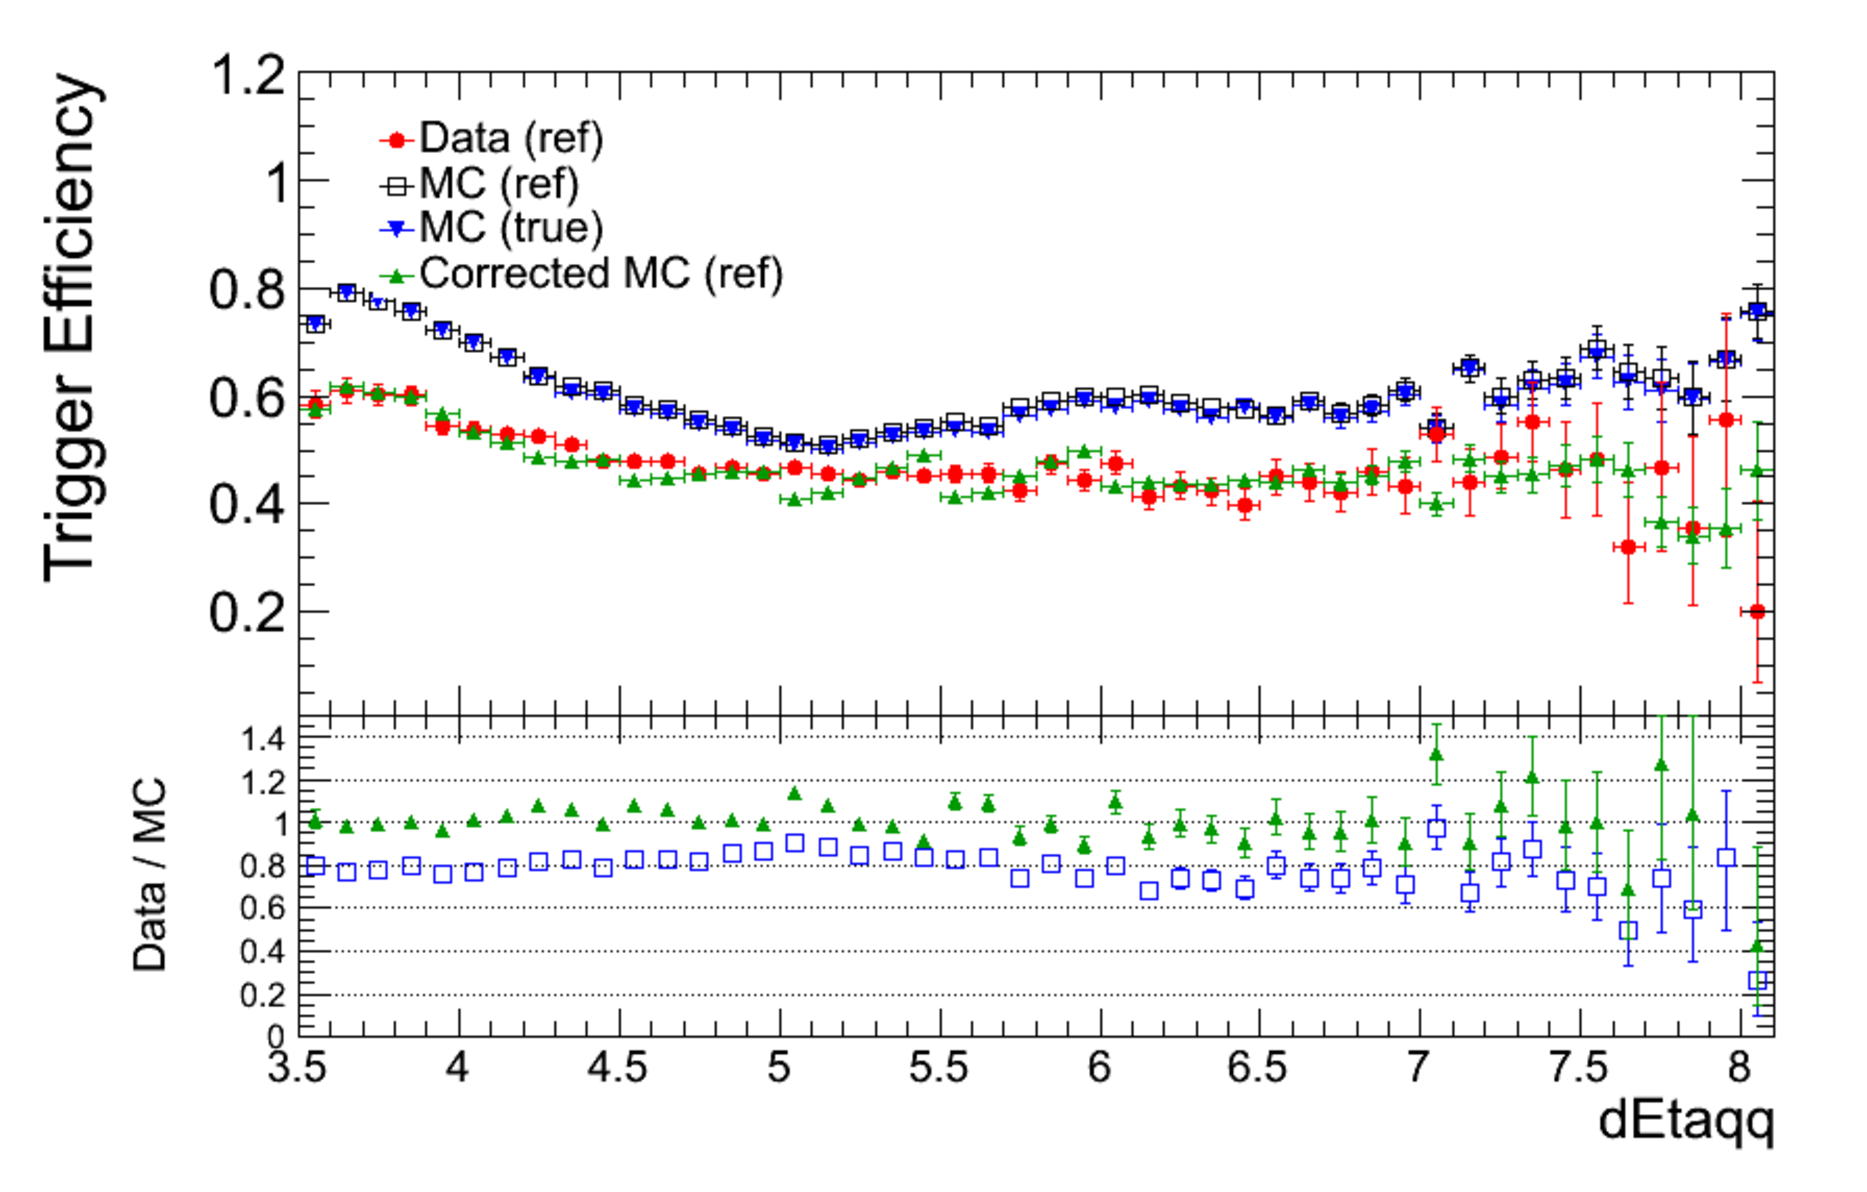
\includegraphics[width=0.45\textwidth]{/home/salderwe/UA/svncontrolled/2013/vbfHbb/vbfHbb_git/latex/Kostas/TrigEff_dEtaqq_VBF.pdf}\hfill
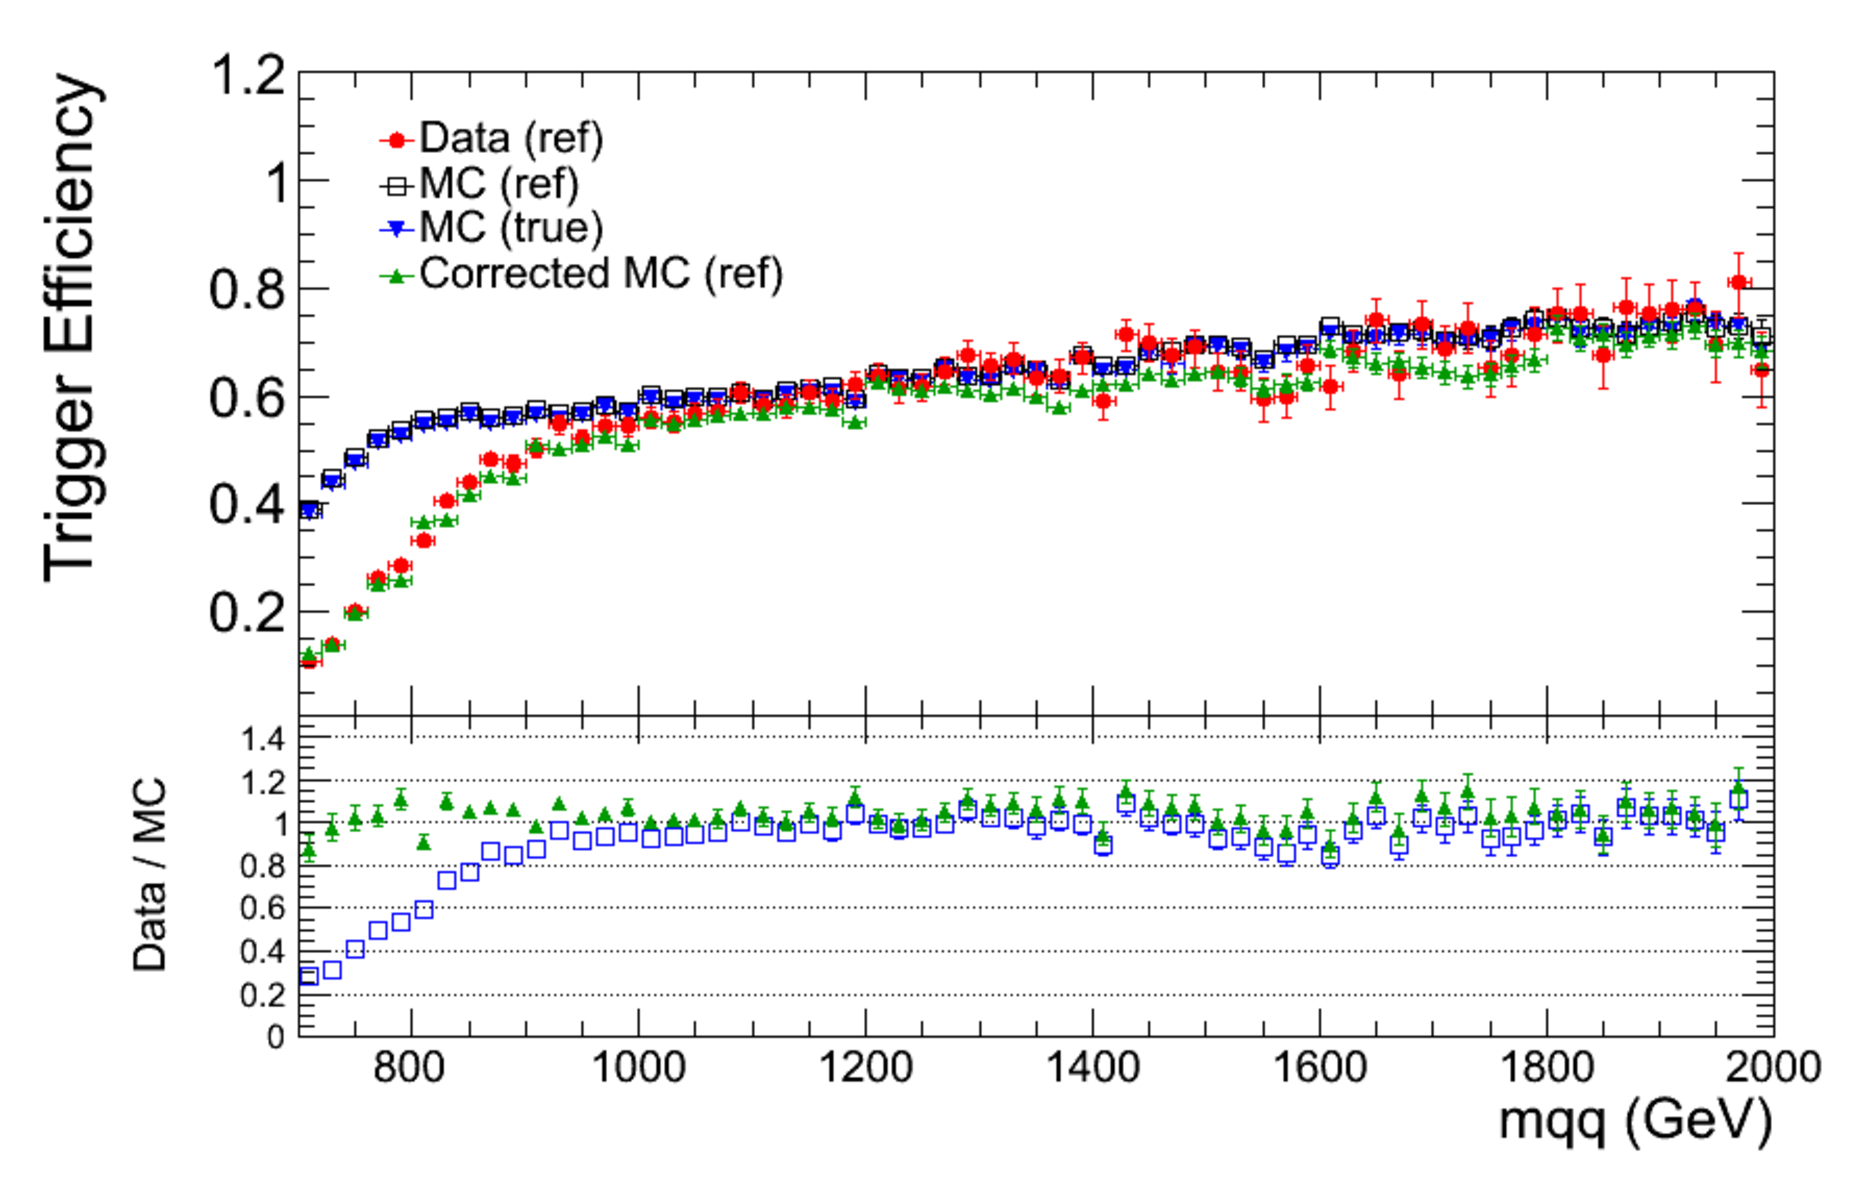
\includegraphics[width=0.45\textwidth]{/home/salderwe/UA/svncontrolled/2013/vbfHbb/vbfHbb_git/latex/Kostas/TrigEff_mqq_VBF.pdf}\vskip 1em
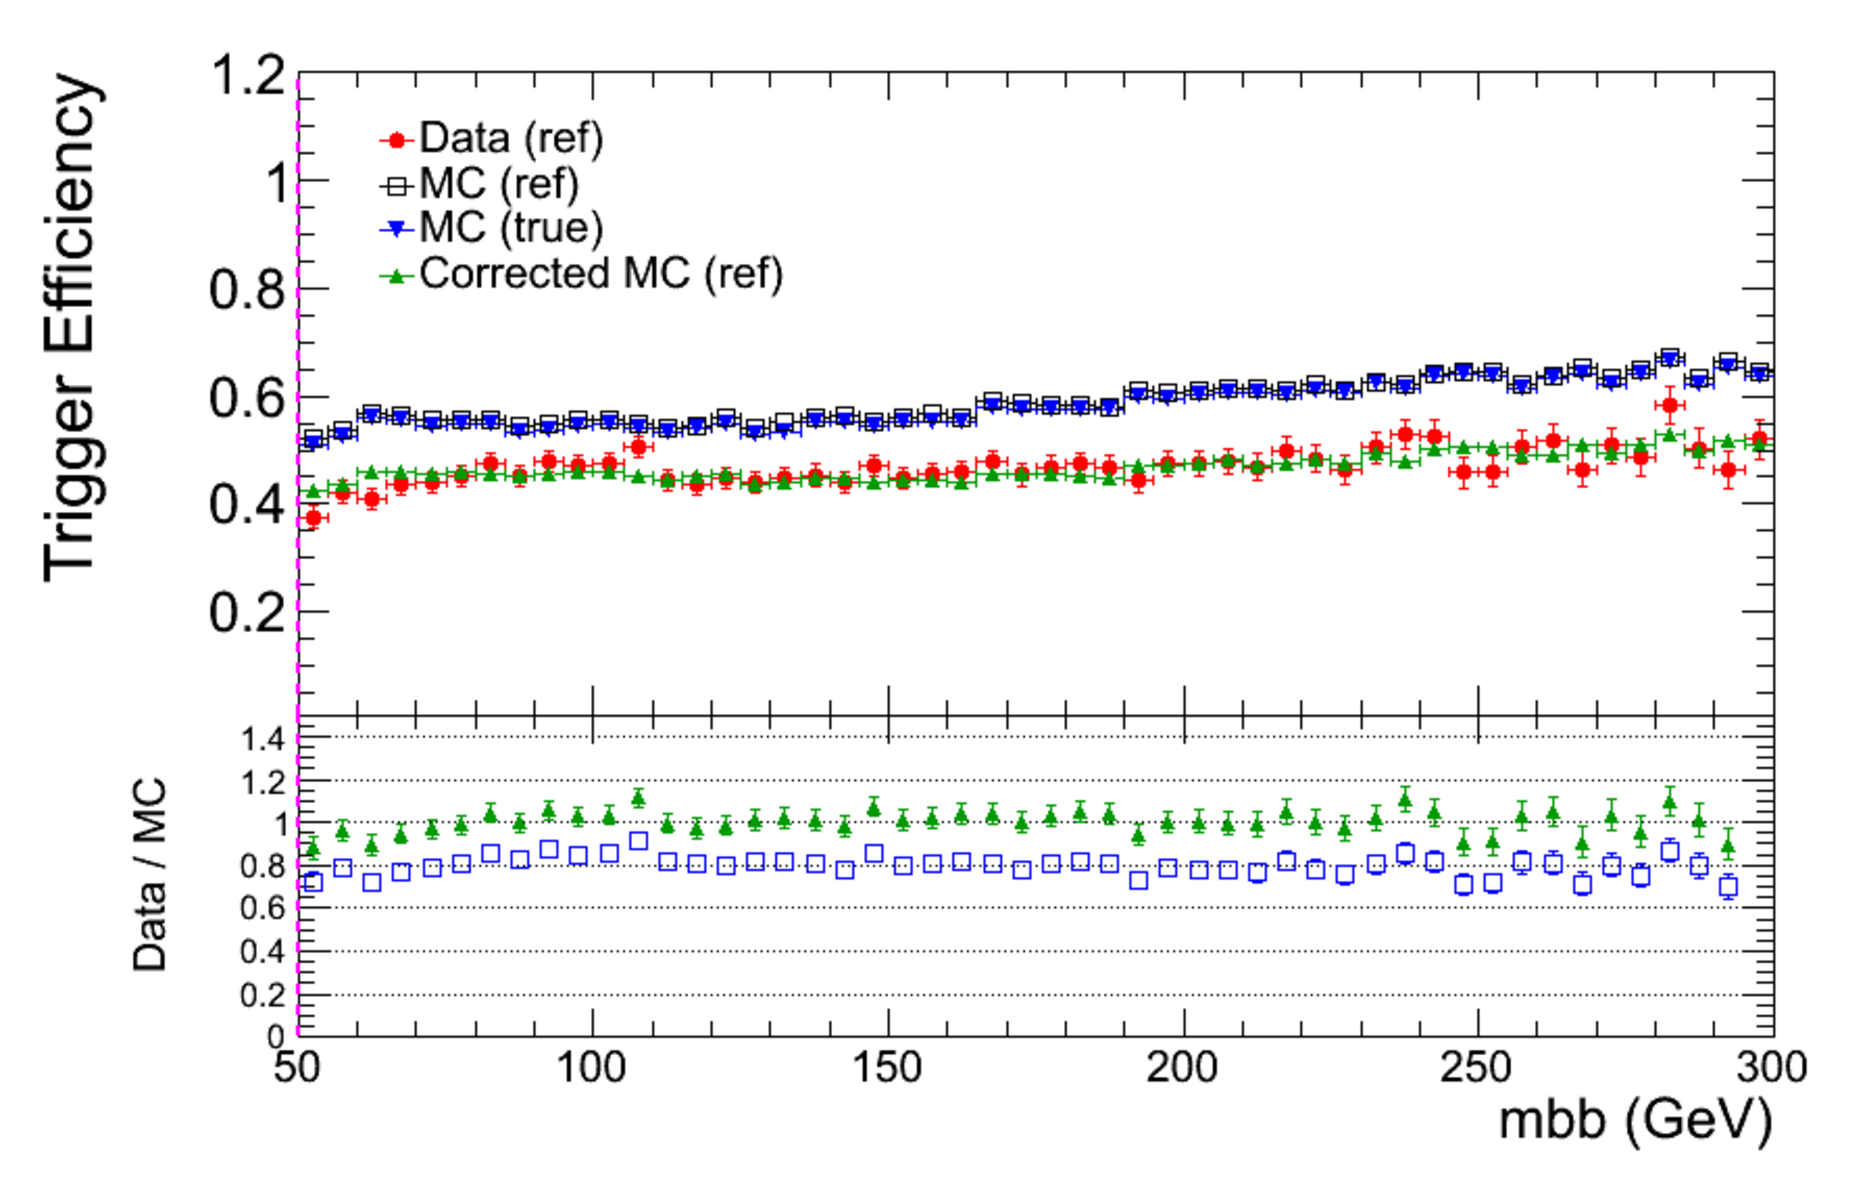
\includegraphics[width=0.45\textwidth]{/home/salderwe/UA/svncontrolled/2013/vbfHbb/vbfHbb_git/latex/Kostas/TrigEff_mbb_VBF.pdf}\hfill
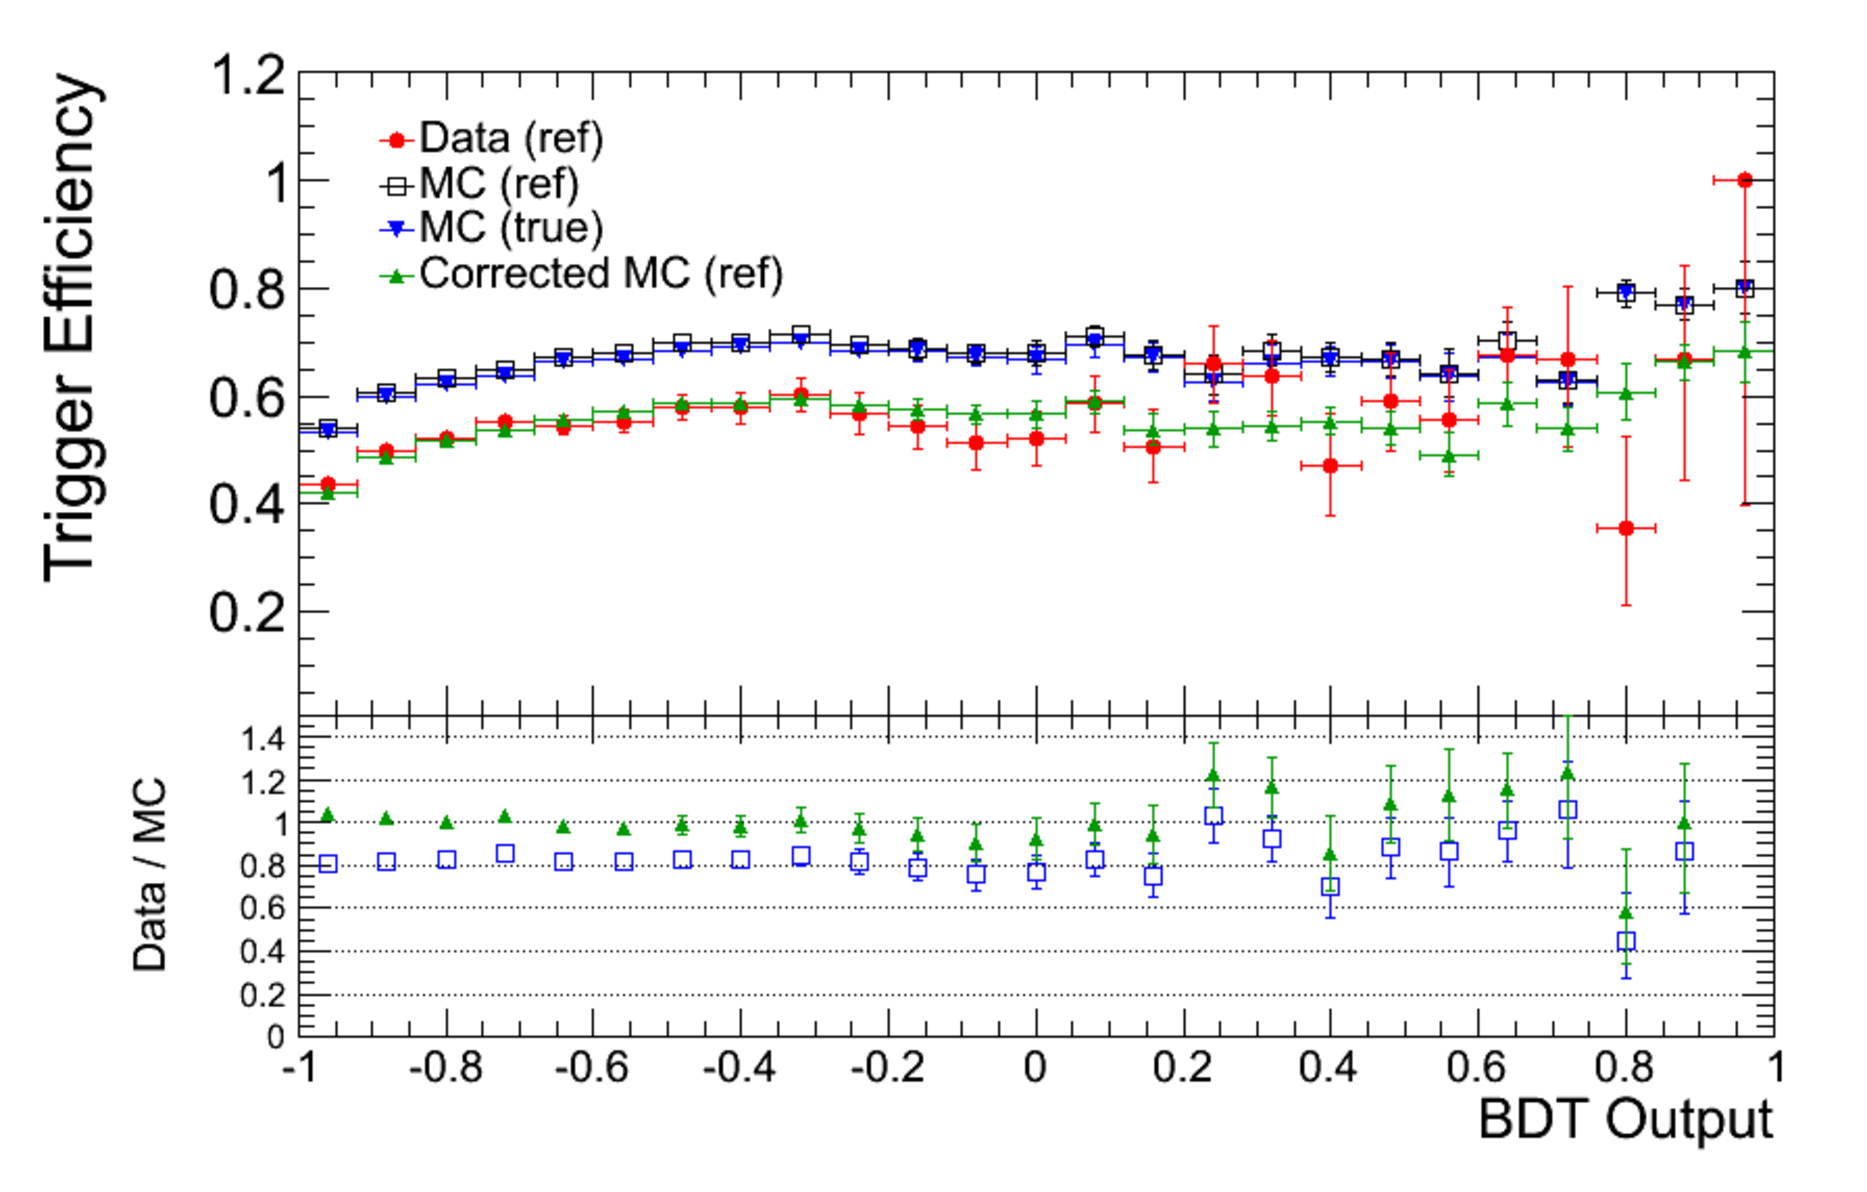
\includegraphics[width=0.45\textwidth]{/home/salderwe/UA/svncontrolled/2013/vbfHbb/vbfHbb_git/latex/Kostas/TrigEff_mva_VBF.pdf}
\end{frame}

%====================================================================================================
\begin{frame}[t,fragile]
\bbl{}\huge NOMINAL
\ebl
\end{frame}

%====================================================================================================
\begin{frame}[t,fragile]{reference trigger AV80}
\begin{python}
thelist=["/home/salderwe/UA/svncontrolled/2013/vbfHbb/vbfHbb_git/trigger/plots/trigger_Nmin1_20140129_NOM/LUMI-PU.3-XSEC/turnonCurves/global_global/sdEtaqq1_gt2p5-jetPt0_gt80-jetPt1_gt70-jetPt2_gt50-jetPt3_gt40-mqq1_gt250_tNOMMC/t_dEtaqq1-B21-2-9_global_global_sdEtaqq1_gt2p5-jetPt0_gt80-jetPt1_gt70-jetPt2_gt50-jetPt3_gt40-mqq1_gt250_tNOMMC_dNOM_rAV80.png","/home/salderwe/UA/svncontrolled/2013/vbfHbb/vbfHbb_git/trigger/plots/trigger_Nmin1_20140129_NOM/LUMI-PU.3-XSEC/turnonCurves/global_global/sdEtaqq1_gt2p5-jetPt0_gt80-jetPt1_gt70-jetPt2_gt50-jetPt3_gt40-mqq1_gt250_tNOMMC/t_jetPt0-B20-0-400_global_global_sdEtaqq1_gt2p5-jetPt0_gt80-jetPt1_gt70-jetPt2_gt50-jetPt3_gt40-mqq1_gt250_tNOMMC_dNOM_rAV80.png","/home/salderwe/UA/svncontrolled/2013/vbfHbb/vbfHbb_git/trigger/plots/trigger_Nmin1_20140129_NOM/LUMI-PU.3-XSEC/turnonCurves/global_global/sdEtaqq1_gt2p5-jetPt0_gt80-jetPt1_gt70-jetPt2_gt50-jetPt3_gt40-mqq1_gt250_tNOMMC/t_jetPt1-B15-0-300_global_global_sdEtaqq1_gt2p5-jetPt0_gt80-jetPt1_gt70-jetPt2_gt50-jetPt3_gt40-mqq1_gt250_tNOMMC_dNOM_rAV80.png","/home/salderwe/UA/svncontrolled/2013/vbfHbb/vbfHbb_git/trigger/plots/trigger_Nmin1_20140129_NOM/LUMI-PU.3-XSEC/turnonCurves/global_global/sdEtaqq1_gt2p5-jetPt0_gt80-jetPt1_gt70-jetPt2_gt50-jetPt3_gt40-mqq1_gt250_tNOMMC/t_jetPt2-B40-0-200_global_global_sdEtaqq1_gt2p5-jetPt0_gt80-jetPt1_gt70-jetPt2_gt50-jetPt3_gt40-mqq1_gt250_tNOMMC_dNOM_rAV80.png","/home/salderwe/UA/svncontrolled/2013/vbfHbb/vbfHbb_git/trigger/plots/trigger_Nmin1_20140129_NOM/LUMI-PU.3-XSEC/turnonCurves/global_global/sdEtaqq1_gt2p5-jetPt0_gt80-jetPt1_gt70-jetPt2_gt50-jetPt3_gt40-mqq1_gt250_tNOMMC/t_jetPt3-B40-0-150_global_global_sdEtaqq1_gt2p5-jetPt0_gt80-jetPt1_gt70-jetPt2_gt50-jetPt3_gt40-mqq1_gt250_tNOMMC_dNOM_rAV80.png","/home/salderwe/UA/svncontrolled/2013/vbfHbb/vbfHbb_git/trigger/plots/trigger_Nmin1_20140129_NOM/LUMI-PU.3-XSEC/turnonCurves/global_global/sdEtaqq1_gt2p5-jetPt0_gt80-jetPt1_gt70-jetPt2_gt50-jetPt3_gt40-mqq1_gt250_tNOMMC/t_mqq1-B75-0-3000_global_global_sdEtaqq1_gt2p5-jetPt0_gt80-jetPt1_gt70-jetPt2_gt50-jetPt3_gt40-mqq1_gt250_tNOMMC_dNOM_rAV80.png"]

for iimg,img in enumerate(sorted(thelist)):
  print r'\includegraphics[width=0.3\textwidth]{%s}'%img
  if not iimg%3==2: print r'\hfill'
  else: print r'\newline'
  
\end{python}
\end{frame}

%====================================================================================================
\begin{frame}[t,fragile]{reference trigger PF80}
\begin{python}
thelist=["/home/salderwe/UA/svncontrolled/2013/vbfHbb/vbfHbb_git/trigger/plots/trigger_Nmin1_20140129_NOM/LUMI-PU.3-XSEC/turnonCurves/global_global/sdEtaqq1_gt2p5-jetPt0_gt80-jetPt1_gt70-jetPt2_gt50-jetPt3_gt40-mqq1_gt250_tNOMMC/t_mqq1-B75-0-3000_global_global_sdEtaqq1_gt2p5-jetPt0_gt80-jetPt1_gt70-jetPt2_gt50-jetPt3_gt40-mqq1_gt250_tNOMMC_dNOM_rPF80.png","/home/salderwe/UA/svncontrolled/2013/vbfHbb/vbfHbb_git/trigger/plots/trigger_Nmin1_20140129_NOM/LUMI-PU.3-XSEC/turnonCurves/global_global/sdEtaqq1_gt2p5-jetPt0_gt80-jetPt1_gt70-jetPt2_gt50-jetPt3_gt40-mqq1_gt250_tNOMMC/t_dEtaqq1-B21-2-9_global_global_sdEtaqq1_gt2p5-jetPt0_gt80-jetPt1_gt70-jetPt2_gt50-jetPt3_gt40-mqq1_gt250_tNOMMC_dNOM_rPF80.png","/home/salderwe/UA/svncontrolled/2013/vbfHbb/vbfHbb_git/trigger/plots/trigger_Nmin1_20140129_NOM/LUMI-PU.3-XSEC/turnonCurves/global_global/sdEtaqq1_gt2p5-jetPt0_gt80-jetPt1_gt70-jetPt2_gt50-jetPt3_gt40-mqq1_gt250_tNOMMC/t_jetPt0-B20-0-400_global_global_sdEtaqq1_gt2p5-jetPt0_gt80-jetPt1_gt70-jetPt2_gt50-jetPt3_gt40-mqq1_gt250_tNOMMC_dNOM_rPF80.png","/home/salderwe/UA/svncontrolled/2013/vbfHbb/vbfHbb_git/trigger/plots/trigger_Nmin1_20140129_NOM/LUMI-PU.3-XSEC/turnonCurves/global_global/sdEtaqq1_gt2p5-jetPt0_gt80-jetPt1_gt70-jetPt2_gt50-jetPt3_gt40-mqq1_gt250_tNOMMC/t_jetPt1-B15-0-300_global_global_sdEtaqq1_gt2p5-jetPt0_gt80-jetPt1_gt70-jetPt2_gt50-jetPt3_gt40-mqq1_gt250_tNOMMC_dNOM_rPF80.png","/home/salderwe/UA/svncontrolled/2013/vbfHbb/vbfHbb_git/trigger/plots/trigger_Nmin1_20140129_NOM/LUMI-PU.3-XSEC/turnonCurves/global_global/sdEtaqq1_gt2p5-jetPt0_gt80-jetPt1_gt70-jetPt2_gt50-jetPt3_gt40-mqq1_gt250_tNOMMC/t_jetPt2-B40-0-200_global_global_sdEtaqq1_gt2p5-jetPt0_gt80-jetPt1_gt70-jetPt2_gt50-jetPt3_gt40-mqq1_gt250_tNOMMC_dNOM_rPF80.png","/home/salderwe/UA/svncontrolled/2013/vbfHbb/vbfHbb_git/trigger/plots/trigger_Nmin1_20140129_NOM/LUMI-PU.3-XSEC/turnonCurves/global_global/sdEtaqq1_gt2p5-jetPt0_gt80-jetPt1_gt70-jetPt2_gt50-jetPt3_gt40-mqq1_gt250_tNOMMC/t_jetPt3-B40-0-150_global_global_sdEtaqq1_gt2p5-jetPt0_gt80-jetPt1_gt70-jetPt2_gt50-jetPt3_gt40-mqq1_gt250_tNOMMC_dNOM_rPF80.png"]

for iimg,img in enumerate(sorted(thelist)):
  print r'\includegraphics[width=0.3\textwidth]{%s}'%img
  if not iimg%3==2: print r'\hfill'
  else: print r'\newline'

\end{python}
\end{frame}

%====================================================================================================
% \begin{frame}[t,fragile]
% \tiny\begin{Verbatim}
% MAPS:
% ../common/main.py -d -D "../common/vbfHbb_defaultOpts_2013.json" -G "/windows/Users/Sara/Desktop/UAData/autumn2013" -t "VBF" --datatrigger "VBF" -s "JetMon,QCD" -p "run194270;jetPt3_gt30;jetPtAve_gt80" -r "AV80" -w "18281.,PU#3;XSEC;LUMI" -o "rootfiles/trigger_2DMap_20140128.root" -m "mqq2;600#700#750#800#850#900#950#1000#1050#1100#1200#1400#1600#1800#2000#2500#3000,dEtaqq2;3.5#3.8#4.0#4.5#5.0#5.5#6.0#6.5#7.0#10.0"
% 
% 
% TRIGGER: UNCORRECTED (CLOSURE)
% ./mkTurnonCurves.py -d -D "../common/vbfHbb_defaultOpts_2013.json" -G "/windows/Users/Sara/Desktop/UAData/autumn2013" -t "VBF" --datatrigger "VBF" --binning "mqq2;75;0;3000,mbb2;30;0;300,ht;75;0;1500,dEtaqq2;21;2;9,mbbReg2;30;0;300,jetPt0;20;0;400,jetPt1;15;0;300,mvaVBF;10;-1;1,mjjTrig;75;0;3000,dEtaTrig;21;2;9,ptAve;50;0;500" -s "QCD" -p "run194270;jetPt3_gt30;mqq2_gt700;mjjTrig_gt700;dEtaqq2_gt3p5;dEtaTrig_gt3p5;jetPtAve_gt80" -v "mqq2,mjjTrig,dEtaqq2,dEtaTrig,mbbReg2,mvaVBF,jetPt0,jetPt1,ptAve" -r "None" -w "18281.,PU#3;XSEC;LUMI,,,rootfiles/trigger_2DMap_20140128.root;2DMaps/JetMon-QCD/2DMap_JetMon-QCD-Rat_sjetPt3_gt30-jetPtAve_gt80-run194270-tVBF-rAV80-dVBF_mqq2-dEtaqq2" --fill -o "rootfiles/trigger_Nmin1_20140128.root"
% 
% ./mkTurnonCurves.py -d -D "../common/vbfHbb_defaultOpts_2013.json" -G "/windows/Users/Sara/Desktop/UAData/autumn2013" -t "VBF" --datatrigger "VBF" --binning "mqq2;75;0;3000,mbb2;30;0;300,ht;75;0;1500,dEtaqq2;21;2;9,mbbReg2;30;0;300,jetPt0;20;0;400,jetPt1;15;0;300,mvaVBF;10;-1;1,mjjTrig;75;0;3000,dEtaTrig;21;2;9,ptAve;50;0;500" -s "JetMon,QCD" -p "run194270;jetPt3_gt30;mqq2_gt700;mjjTrig_gt700;dEtaqq2_gt3p5;dEtaTrig_gt3p5;jetPtAve_gt80" -v "mqq2,mjjTrig,dEtaqq2,dEtaTrig,mbbReg2,mvaVBF,jetPt0,jetPt1,ptAve" -r "AV80" -w "18281.,PU#3;XSEC;LUMI,,,rootfiles/trigger_2DMap_20140128.root;2DMaps/JetMon-QCD/2DMap_JetMon-QCD-Rat_sjetPt3_gt30-jetPtAve_gt80-run194270-tVBF-rAV80-dVBF_mqq2-dEtaqq2" --drawstack --closure --shade -o "rootfiles/trigger_Nmin1_20140128.root"
% 
% 
% TRIGGER: CORRECTED
% ./mkTurnonCurves.py -d -D "../common/vbfHbb_defaultOpts_2013.json" -G "/windows/Users/Sara/Desktop/UAData/autumn2013" -t "VBF" --datatrigger "VBF" --binning "mqq2;75;0;3000,mbb2;30;0;300,ht;75;0;1500,dEtaqq2;21;2;9,mbbReg2;30;0;300,jetPt0;20;0;400,jetPt1;15;0;300,mvaVBF;10;-1;1,mjjTrig;75;0;3000,dEtaTrig;21;2;9,ptAve;50;0;500" -s "JetMon,QCD" -p "run194270;jetPt3_gt30;mqq2_gt700;mjjTrig_gt700;dEtaqq2_gt3p5;dEtaTrig_gt3p5;jetPtAve_gt80" -v "mqq2,mjjTrig,dEtaqq2,dEtaTrig,mbbReg2,mvaVBF,jetPt0,jetPt1,ptAve" -r "AV80" -w "18281.,PU#3;XSEC;LUMI;MAP#mqq[2]#dEtaqq[2],,,rootfiles/trigger_2DMap_20140128.root;2DMaps/JetMon-QCD/2DMap_JetMon-QCD-Rat_sjetPt3_gt30-jetPtAve_gt80-run194270-tVBF-rAV80-dVBF_mqq2-dEtaqq2" --drawstack --overlay --shade -o "rootfiles/trigger_Nmin1_20140128.root"
% 
% 
% CONTROL: UNCORRECTED
% ./mkHist.py -D "../common/vbfHbb_defaultOpts_2013.json" -G "/windows/Users/Sara/Desktop/UAData/autumn2013" -t "VBF" --datatrigger "VBF" --binning "mqq2;75;0;3000,mbb2;30;0;300,mjjTrig;75;0;3000,mbb1;30;0;300,ht;75;0;1500,dEtaqq2;21;2;9,mbbReg2;30;0;300,dEtaqq1;60;2;8,mbbReg1;30;0;300,jetPt0;40;0;400,jetPt1;30;0;300,mvaVBF;20;-1;1,ptAve;50;0;500,dEtaTrig;21;2;9" --nosample "JetMon,VBF115,VBF120,VBF130,VBF135,DataA,DataB,DataC,DataD" -d -K -p "dEtaqq2_gt3p5;dEtaTrig_gt3p5;mqq2_gt700;mjjTrig_gt700;dPhibb2_lt2;nLeptons;Btag0_ML;NOMtrgveto;jetPt3_gt30;jetPtAve_gt80" -v "jetPt0,jetPt1,mjjTrig,dEtaTrig,mvaVBF,mqq2,dEtaqq2,ptAve,mbbReg2" -w "18281.,XSEC;LUMI;KFAC;PU#0,,1.610797,../trigger/rootfiles/trigger_2DMap_20140128.root;2DMaps/JetMon-QCD/2DMap_JetMon-QCD-Rat_sjetPt3_gt30-jetPtAve_gt80-run194270-tVBF-rAV80-dVBF_mqq2-dEtaqq2" --drawstack -o "rootfiles/controlPlots_20140128.root"
% 
% 
% CONTROL: CORRECTED
% ./mkHist.py -D "../common/vbfHbb_defaultOpts_2013.json" -G "/windows/Users/Sara/Desktop/UAData/autumn2013" -t "VBF" --datatrigger "VBF" --binning "mqq2;75;0;3000,mbb2;30;0;300,mjjTrig;75;0;3000,mbb1;30;0;300,ht;75;0;1500,dEtaqq2;21;2;9,mbbReg2;30;0;300,dEtaqq1;60;2;8,mbbReg1;30;0;300,jetPt0;40;0;400,jetPt1;30;0;300,mvaVBF;20;-1;1,ptAve;50;0;500,dEtaTrig;21;2;9" --nosample "JetMon,VBF115,VBF120,VBF130,VBF135,DataA,DataB,DataC,DataD" -d -K -p "dEtaqq2_gt3p5;dEtaTrig_gt3p5;mqq2_gt700;mjjTrig_gt700;dPhibb2_lt2;nLeptons;Btag0_ML;NOMtrgveto;jetPt3_gt30;jetPtAve_gt80" -v "mqq2,dEtaqq2,mbbReg2,ptAve,mvaVBF,jetPt0,jetPt1,mjjTrig,dEtaTrig" -w "18281.,XSEC;LUMI;KFAC;PU#0;MAP#mqq[2]#dEtaqq[2],,2.019084,../trigger/rootfiles/trigger_2DMap_20140128.root;2DMaps/JetMon-QCD/2DMap_JetMon-QCD-Rat_sjetPt3_gt30-jetPtAve_gt80-run194270-tVBF-rAV80-dVBF_mqq2-dEtaqq2" --drawstack -o "rootfiles/controlPlots_20140128.root"
% 
% \end{Verbatim}
% \end{frame}

%====================================================================================================
\end{document}

